\input qpd-bootstrap

\begin{problem}{20260815}
  \meta{name}{Optimization}
  \meta{setter}{Andy He}
  \meta{score}{4}
  \meta{topic}{Mechanics}
  \meta{difficulty}{1}
  \meta{tags}{}
  \meta{open}{true}
  \meta{resources}{}                % optional — comma-separated allowed resources

  柳如烟天天刷AP题，并且坚信只要她每天都刷100套SAT她侄子张耀祖就能获得天生CB圣体，并且像某位可爱的同学一样三天学完世界史。但是岳父岳母觉得现在是AI时代，应该用AI解题。柳如烟觉得很有道理，决定每天用AI做100套SAT，张耀祖平安地出生了，但是柳如烟发现张耀祖居然只会用AI解题，觉得一定是自己之前用AI的原因，所以恨毒了岳父岳母，一通电话给他们约上天台，准备把他们踢下去。然后在天台上，柳如烟在试图踹下岳父岳母时发现他们其实是奥特曼，所以在一番纠缠之下他们三个以速度V与水平相比仰角角度Phi飞出了高h米的大楼，然后我用他们的遗产买了一套大平层从此开心地活了下去。这次，柳如烟重生了，于是她开始手算AP题，她遇到的第一题就是她死前最后的念想:同样的速度V,phi为多大时(Indegrees),她们三个飞的最远(水平)。

  \begin{center}
    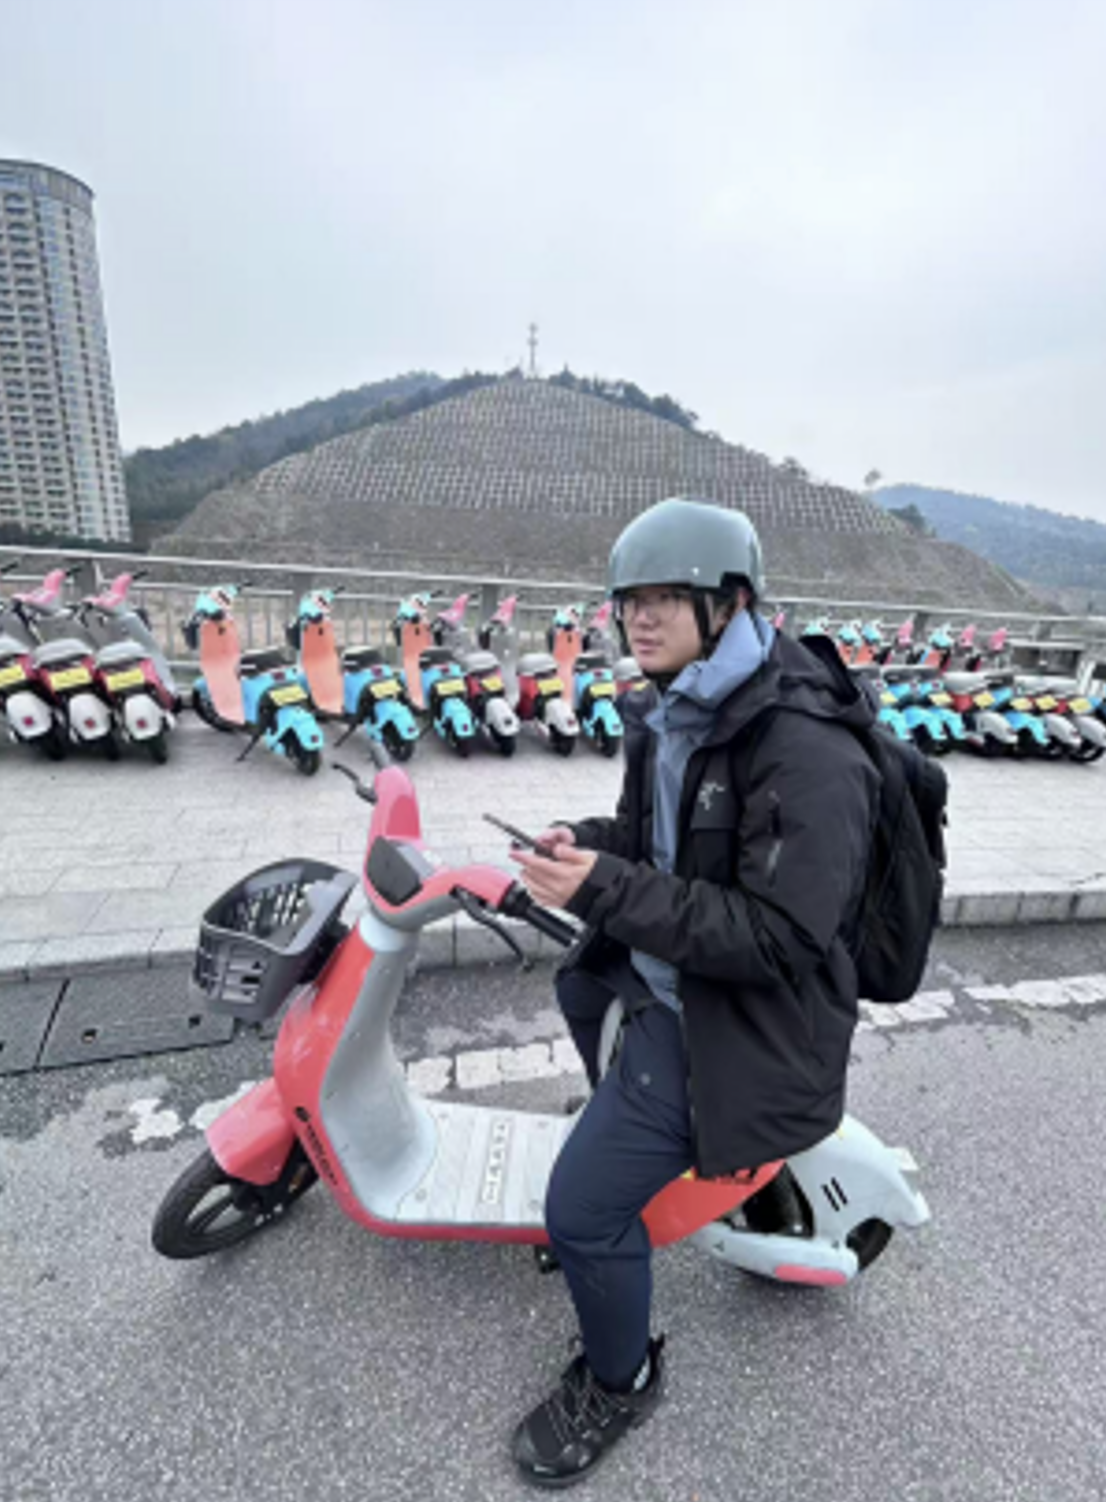
\includegraphics[width=0.45\linewidth]{assets/20260815-1.png}
    \caption{}
  \end{center}
\end{problem}

\begin{solution}{YYYYMMDD}
  % Solution goes here.  One \subsection*{Qn. Title} per question.
  %
  %   \subsection*{Q1. First question title}
  %   ...
  %
  % Available environments:
  %   \begin{assumption}    ...        \end{assumption}
  %   \begin{answer}        ...        \end{answer}
\end{solution}

\input qpd-end
